%==========================
% Chapter 4: High-Dimensional Representations
%==========================

\chapter{High-Dimensional Representations}

\begin{keyinsight}
High-dimensional spaces are strange. Random vectors are nearly orthogonal. Most of the volume of a high-dimensional ball is concentrated near its surface. Distances become uniform. These counterintuitive properties are not bugs, they are features. Understanding high-dimensional geometry is essential for working with embeddings, vectors, and similarity search in modern AI systems.
\end{keyinsight}

\vspace{1.5em}

In the previous chapters, we built foundations in information theory, Bayesian inference, and geometric thinking. Now we turn to a practical question: how do we represent data in high-dimensional spaces?

Modern AI systems work with embeddings. Text becomes vectors. Images become vectors. Everything becomes vectors living in spaces with hundreds or thousands of dimensions. These vectors encode semantic meaning: similar concepts have similar vectors, measured by distances or angles.

But high-dimensional spaces behave very differently from the two- or three-dimensional spaces we experience in daily life. Intuitions break down. Distances become less meaningful. Random vectors are surprisingly close to orthogonal. The geometry has unusual properties that you must understand to work effectively with these representations.

This chapter teaches you the essential phenomena of high-dimensional geometry. We start with concentration of measure: how probability mass concentrates in surprising ways as dimensions increase. Then we explore random projections and the Johnson--Lindenstrauss lemma, which tells you that you can compress high-dimensional data with minimal distortion. We will dive into tokenization and embedding geometry, understanding why embeddings often suffer from anisotropy and how whitening can fix it. Finally, we will look at spherical codes and similarity search, seeing how information theory connects to the practical problem of finding nearest neighbors.

Throughout, we will see concrete examples and practical techniques. High-dimensional geometry is not just abstract mathematics. It determines how well your retrieval system works, how efficiently you can search large databases, and how faithfully your embeddings capture semantic relationships.

\vspace{2em}

%==========================
\section{Concentration of Measure: The Geometry of High Dimensions}

\subsection{The Curse and Blessing of Dimensionality}

You have probably heard of the "curse of dimensionality." As dimensions increase, the number of cells in a fixed-resolution grid grows exponentially, so the number of data points you need to fill a space explodes. Distances become less discriminative. Nearest neighbor search becomes harder.

This is all true, but there is another side. High dimensions also give you blessings. Random vectors are nearly orthogonal, which means you can pack many almost independent directions into a space. Concentration phenomena mean that probability mass concentrates tightly, which makes some calculations easier. Random projections preserve distances, which means you can compress without losing much information.

\vspace{1em}

Understanding both the curse and the blessing is essential. High dimensions are different, but different does not mean bad. You need to work with the geometry, not against it.

\vspace{0.5em}

\textbf{The blessing side (in brief).} When distributions are roughly isotropic, three useful effects emerge:

\begin{notationbox}
\textbf{Isotropic (informal).} A distribution in $\mathbb{R}^d$ is isotropic if it has no preferred direction: after centering and scaling, $\operatorname{Cov}(x) \approx I$ (up to an overall scale).

\textbf{Lipschitz.} A function $f$ is $L$-Lipschitz if $|f(x) - f(y)| \le L\|x-y\|$. Many geometric quantities on the unit sphere are $O(1)$-Lipschitz, which is why they concentrate in high dimensions.
\end{notationbox}

\begin{itemize}
\item \emph{Near-orthogonality:} Random directions have tiny correlations ($\mathbb{E}[u^\top v]=0$, $\operatorname{Var}(u^\top v)=1/d$ for independent uniform-on-sphere $u,v$), which simplifies analysis and enables compression via random projections (Sections~\ref{sec:jl}--\ref{sec:jl-proof}).
\item \emph{Concentration in thin shells:} Norms and other Lipschitz functions concentrate, so averages stabilize quickly (Sections ``Most Volume Is Near the Surface'' and ``Typicality and the Thin Shell'').
\item \emph{Low effective dimension:} Many datasets occupy lower-dimensional structure inside a high-dimensional ambient space; exploiting this is a separate blessing (not implied by isotropy) and is central to embeddings and fast retrieval (``Why ANN Works Despite the Curse of Dimensionality'').
\end{itemize}

We will call out both the curses and the blessings as we go, and we will be precise about the distributional assumptions they require.

\vspace{1.5em}

\subsection{Most Volume Is Near the Surface}

Let me start with a striking fact. Consider a ball of radius $r$ in $d$ dimensions. Most of its volume is concentrated in a thin shell near the surface. The center is nearly empty.

To see this, compare the volume of a ball of radius $r$ to the volume of a ball of radius $(1 - \epsilon)r$ for small $\epsilon$:

\begin{equation}
\frac{\text{Volume}(r(1-\epsilon))}{\text{Volume}(r)} = (1-\epsilon)^d
\end{equation}

For large $d$, this ratio goes to zero rapidly. Even for $\epsilon = 0.1$ (removing just the outer 10\% of the radius), if $d = 100$ then $(0.9)^{100} \approx 0.000027$. Almost all the volume is in the outer 10\% shell.

\begin{figure}[t]
\centering
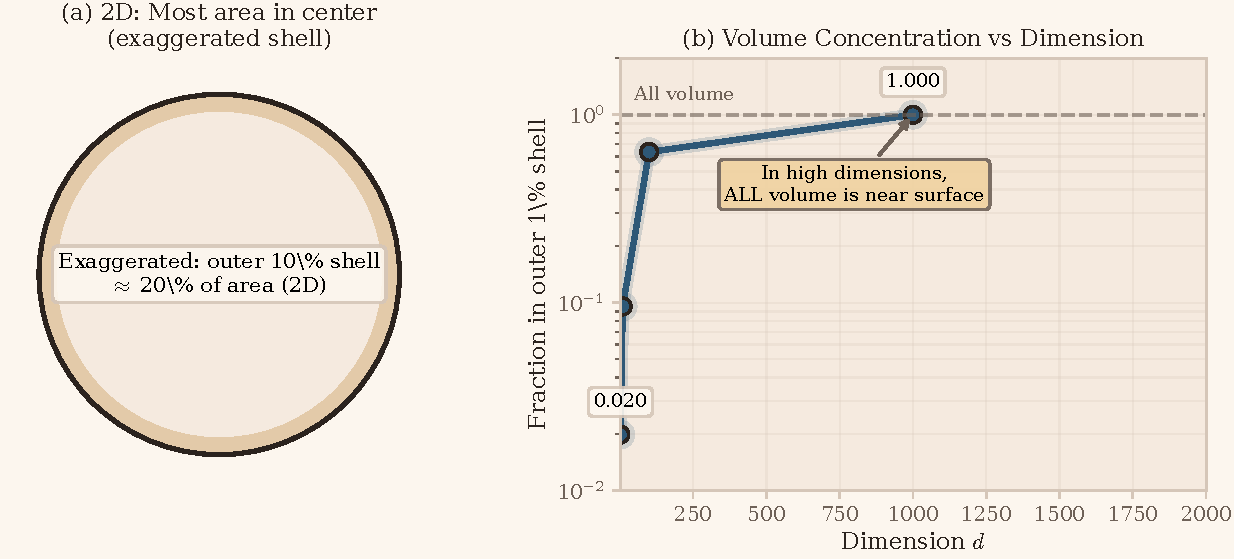
\includegraphics[width=\linewidth]{code/figures/ch04_highdim_representations/fig_4_1_volume_concentration.pdf}
\caption{Most volume lies near the surface in high dimensions: (a) a 2D schematic with an exaggerated outer 10\% shell (for visibility; $\approx$20\% of area in 2D); (b) the fraction of mass in the outer 1\% shell approaches 1 rapidly as dimension grows.}
\label{fig:volume_concentration}
\end{figure}

\vspace{1.5em}

\begin{examplebox}
\textbf{Where is the volume in high dimensions?}

\vspace{0.5em}

Consider a ball of radius 1 in $d$ dimensions. What fraction of the volume is contained within radius $0.99$?

\vspace{0.5em}

The ratio is $(0.99)^d$. Let me compute this for different dimensions:

\begin{itemize}
\item $d = 2$: $(0.99)^2 = 0.98$. About 98\% of the area is within radius 0.99. The center contains significant mass.

\item $d = 10$: $(0.99)^{10} \approx 0.904$. About 90\% of the volume is within radius 0.99. Still reasonable.

\item $d = 100$: $(0.99)^{100} \approx 0.366$. Only 37\% of the volume is within radius 0.99. Most of the volume is in the outer 1\% shell.

\item $d = 1000$: $(0.99)^{1000} \approx 0.00004$. Essentially all the volume is concentrated near the surface. The interior is empty.
\end{itemize}

\vspace{0.5em}

This is deeply counterintuitive. In three dimensions, we think of balls as solid objects with mass throughout. But in high dimensions, balls are hollow shells. The center is empty. Under uniform sampling, almost all the probability mass lies near the surface.

\vspace{0.5em}

\textbf{Practical implication:} If you sample uniformly from a high-dimensional ball, your samples will almost always be near the surface, not near the center. If you later normalize vectors to unit length (project onto the sphere), you often are not discarding much radial information because the mass was already near the boundary.
\end{examplebox}

\vspace{1.5em}

\vspace{0.5em}

\textbf{Caveat (distribution vs.\ volume).} The calculation above is about \emph{volume} and therefore applies to the \emph{uniform} distribution on the ball. Other distributions behave differently. For example, a standard Gaussian in $\mathbb{R}^d$ concentrates in a thin shell around radius $\sqrt{d}$, not exactly at the boundary of the ball. The ``hollow ball'' phenomenon explains where \emph{volume} lives; probability mass may live elsewhere depending on the sampling distribution.

Take a breath here. Let this sink in. High-dimensional balls are hollow. This is the first strange property of high dimensions.

\vspace{1.5em}

\subsection{Random Vectors Are Nearly Orthogonal}

Here is another surprising fact. If you sample two random vectors uniformly from a high-dimensional sphere, they are almost always nearly orthogonal. The angle between them is close to 90 degrees.

Why? Because the dot product of two random unit vectors has expected value zero and variance that shrinks as $1/d$. So as $d \to \infty$, the dot product concentrates near zero, which means the angle concentrates near 90 degrees.

\vspace{1em}

More precisely, if $u$ and $v$ are independent random unit vectors \emph{uniformly distributed on the sphere} (equivalently, if $u,v$ are Gaussian vectors normalized to unit length), then:

\begin{equation}
\mathbb{E}[u^\top v] = 0 \quad \text{and} \quad \operatorname{Var}(u^\top v) = \frac{1}{d}
\end{equation}

This statement needs the uniform-on-sphere (or normalized Gaussian) assumption; it does not hold for arbitrary concentrated distributions on the sphere (e.g., von Mises--Fisher distributions aligned with a pole).

By concentration on the sphere (a standard result is Lévy's lemma), 1-Lipschitz functions fluctuate by at most $t$ with probability $\lesssim \exp(-c d t^2)$. Since $u \mapsto u^\top v$ is 1-Lipschitz for fixed unit $v$, the dot product is typically on the order of $1/\sqrt{d}$. For $d = 1000$, that means $|u^\top v|$ is usually around $0.03$ (angles very close to $90^\circ$).

\vspace{1.5em}

\begin{examplebox}
\textbf{Orthogonality in high dimensions}

\vspace{0.5em}

Generate two random unit vectors $u$ and $v$ in $d$ dimensions (sample coordinates from a standard Gaussian and normalize). What is the typical value of $u^\top v$?

\vspace{0.5em}

I can compute the expected squared dot product:
\begin{equation*}
\mathbb{E}[(u^\top v)^2] = \mathbb{E}\left[\left(\sum_{i=1}^d u_i v_i\right)^2\right] = \sum_{i=1}^d \mathbb{E}[u_i^2 v_i^2] = \frac{1}{d}
\end{equation*}

So the typical magnitude is $|u^\top v| \approx 1/\sqrt{d}$.

\vspace{0.5em}

For different dimensions:

\begin{itemize}
\item $d = 2$: Typical $|u^\top v| \approx 0.7$. Random vectors can have substantial alignment.

\item $d = 10$: Typical $|u^\top v| \approx 0.316$. They are getting more orthogonal.

\item $d = 100$: Typical $|u^\top v| \approx 0.1$. Nearly orthogonal.

\item $d = 1000$: Typical $|u^\top v| \approx 0.03$. Essentially orthogonal.
\end{itemize}

\vspace{0.5em}

In high dimensions, random vectors are nearly orthogonal. This means you can pack many "independent" directions into a high-dimensional space. Each new random vector is almost orthogonal to all previous ones, so you do not get redundancy.

\vspace{0.5em}

\textbf{Practical implication:} When you create random projections or use random features, you are effectively creating nearly orthogonal directions. This is why random projections work well for dimensionality reduction.
\end{examplebox}

\begin{figure}[t]
\centering
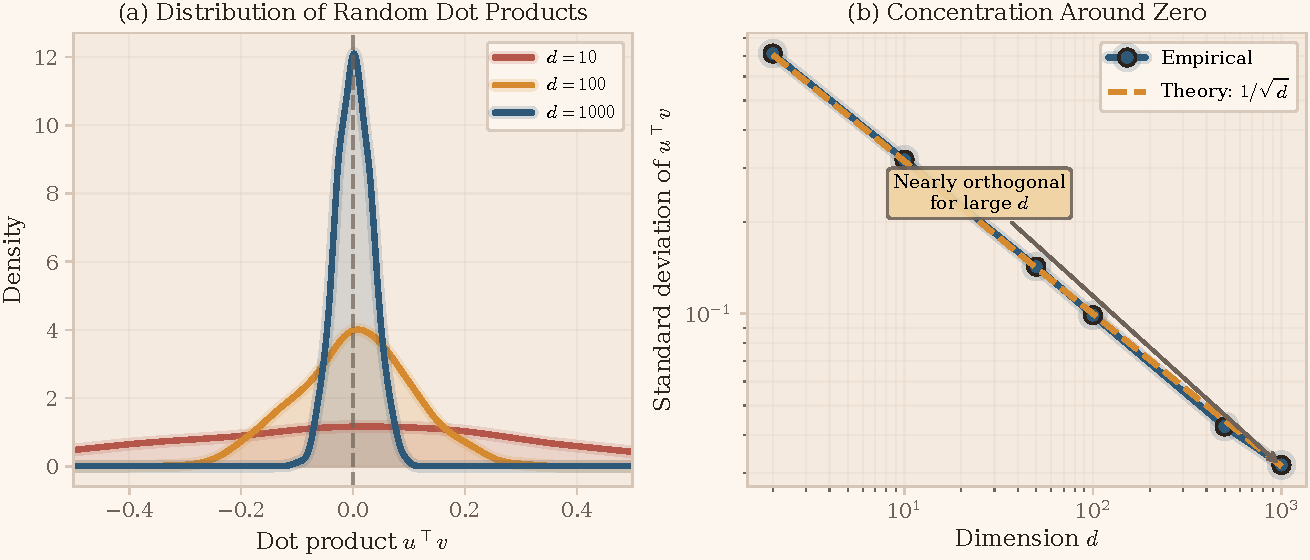
\includegraphics[width=\linewidth]{code/figures/ch04_highdim_representations/fig_4_2_orthogonality.pdf}
\caption{Dot products between random unit vectors concentrate around zero as dimension increases: (a) histograms for $d\in\{10,100,1000\}$; (b) the standard deviation shrinks like $1/\sqrt{d}$.}
\label{fig:orthogonality}
\end{figure}

\vspace{1.5em}

\subsection{Distances Become Uniform}

Here is the third phenomenon. \emph{For many isotropic distributions with concentration,} pairwise distances concentrate around a typical value as dimension grows. A useful rule of thumb is that relative spread shrinks like $O(1/\sqrt{d})$.

For example, if $x,y \sim \mathcal{N}(0, I_d)$, then $x-y \sim \mathcal{N}(0, 2I_d)$ and $\|x-y\|^2 \sim 2\chi^2_d$, so:
\begin{equation}
\mathbb{E}[\|x-y\|^2] = 2d \quad \text{and} \quad \operatorname{Var}(\|x-y\|^2) = 8d,
\end{equation}
which implies the \emph{relative} spread in $\|x-y\|$ decays like $O(1/\sqrt{d})$.

If you have $n$ points sampled i.i.d. from such a distribution and $\log n \ll d$ (equivalently, $n$ is sub-exponential in $d$), then even nearest and farthest distances from a query become hard to distinguish. (The concentration per pair beats the $\log n$ price you pay for taking extrema.) Let $D_{\max}$ be the distance to the farthest point and $D_{\min}$ be the distance to the nearest point. A common summary is:

\begin{equation}
\frac{D_{\max} - D_{\min}}{D_{\min}} \to 0 \quad \text{as } d \to \infty \quad \text{(fixed $n$, isotropic concentration).}
\end{equation}

If $n$ grows like $\exp(\Theta(d))$, this can fail: with astronomically many points, the extreme nearest and farthest neighbors can separate even though typical pairwise distances concentrate.

This is called the concentration of distances. In the worst case, all points become nearly equidistant from a query point, and nearest neighbors and farthest neighbors become hard to separate by raw distance alone.

\begin{figure}[t]
\centering
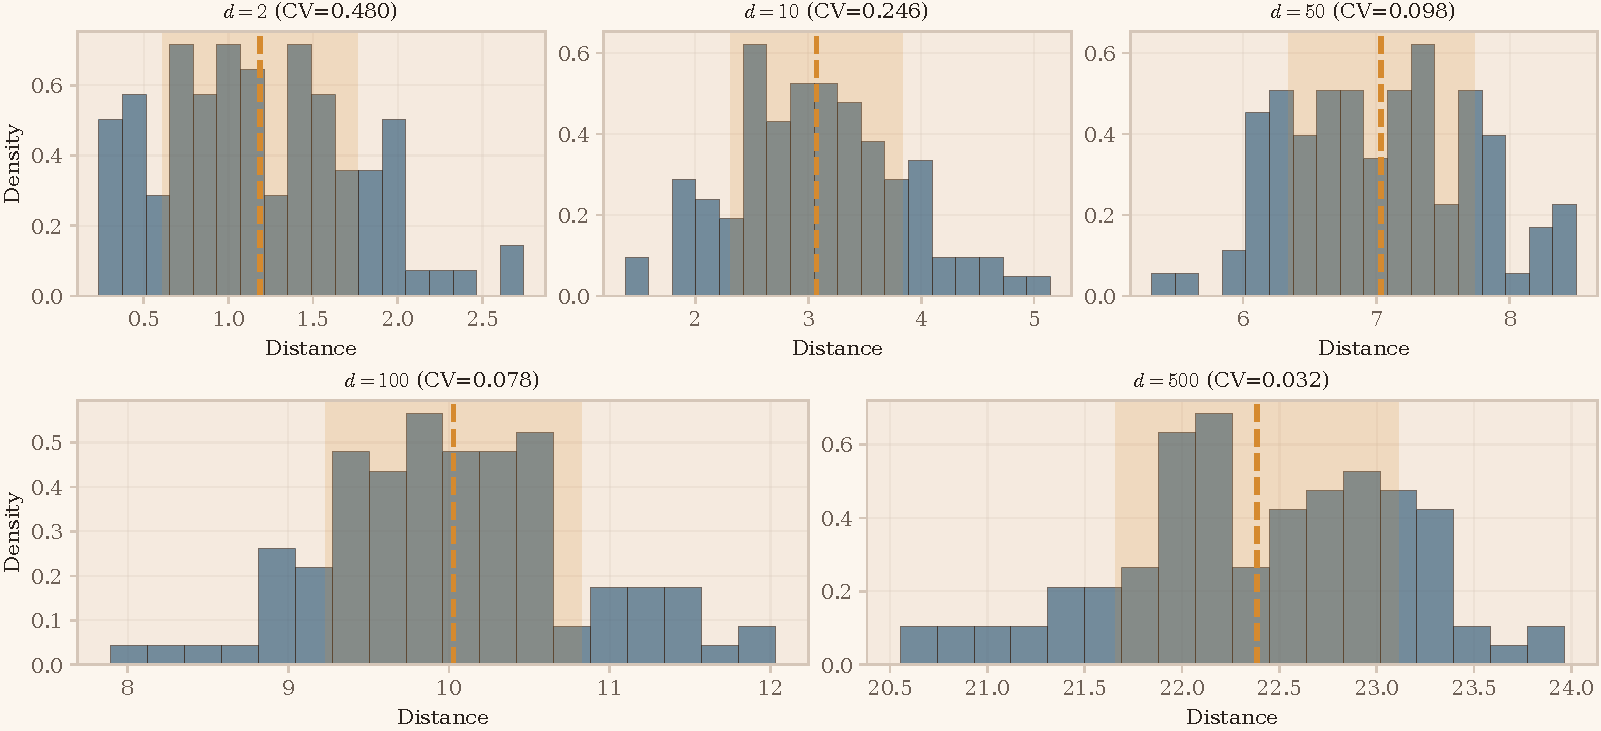
\includegraphics[width=\linewidth]{code/figures/ch04_highdim_representations/fig_4_3_distance_uniformity.pdf}
\caption{Distances become uniform in high dimensions: histograms of radii for Gaussian points show concentration, and the coefficient of variation (std/mean) decreases with $d$.}
\label{fig:distance_uniformity}
\end{figure}

\vspace{1em}

This is a serious problem for nearest neighbor search. If all distances are similar, how do you find the nearest neighbor? The signal (difference between near and far) becomes small relative to the noise (fluctuations in distance).

However, this phenomenon depends on distributional assumptions and on how $n$ scales with $d$. Real data often has structure: it lives on lower-dimensional manifolds embedded in a high-dimensional space, and the geometry can be highly anisotropic. In those cases, distances may remain informative enough that nearest neighbor search (especially approximate search) still works well.

\vspace{1.5em}

\subsection{Typicality and the Thin Shell}

The concentration of measure has a beautiful consequence called typicality. Most samples from a distribution are concentrated in a "typical set" where the probability is neither too high nor too low. The typical set has high probability mass but small volume.

For example, consider a Gaussian distribution in $d$ dimensions. Most samples have norm close to $\sqrt{d}$. They concentrate in a thin shell around radius $\sqrt{d}$. Samples very close to the origin (norm much less than $\sqrt{d}$) or very far from the origin (norm much greater than $\sqrt{d}$) are exponentially rare.

\vspace{1em}

This connects back to information theory. Typicality is a statement about \emph{surprise}: for many distributions, the per-dimension quantity $-\frac{1}{d}\log p(x)$ concentrates near a constant. In discrete i.i.d. models, that constant is the entropy rate $H$ (in bits if you use $\log_2$), so typical samples have code lengths close to $H$. For continuous distributions, read $p(x)$ as a \emph{density}; the analogous constant is the differential entropy rate, and literal bit lengths require quantizing to finite precision. Samples outside the typical set have either much shorter code length/surprise (rare) or much longer code length/surprise (also rare).

\vspace{1em}

Typicality is fundamental to compression and coding. When you design a code, you allocate bits to the typical set. Samples outside the typical set can be coded less efficiently because they are rare anyway.

\vspace{2em}

Let me give you a concrete example to make this real.

\vspace{1.5em}

\begin{examplebox}
\textbf{Typicality of Gaussian samples}

\vspace{0.5em}

Sample $x$ from a standard Gaussian $\mathcal{N}(0, I_d)$ in $d$ dimensions. What is the typical value of $\|x\|^2$?

\vspace{0.5em}

Each coordinate $x_i \sim \mathcal{N}(0, 1)$ is independent. So $\|x\|^2 = \sum_{i=1}^d x_i^2$ is the sum of $d$ independent $\chi^2$ random variables with one degree of freedom each. By the law of large numbers:

\begin{equation*}
\mathbb{E}[\|x\|^2] = d \quad \text{and} \quad \text{Var}(\|x\|^2) = 2d
\end{equation*}

So the typical squared norm is $d$, giving a typical norm of $\sqrt{d}$. The standard deviation of $\|x\|^2$ is $\sqrt{2d}$, which means the standard deviation of $\|x\|$ is approximately $\sqrt{2d}/(2\sqrt{d}) = 1/\sqrt{2}$ (delta method: linearize $\sqrt{\,\cdot\,}$ around the mean and propagate variance).

\vspace{0.5em}

The relative standard deviation in the norm is:
\begin{equation*}
\frac{\text{std}(\|x\|)}{\mathbb{E}[\|x\|]} \approx \frac{1/\sqrt{2}}{\sqrt{d}} = \frac{1}{\sqrt{2d}} \to 0 \text{ as } d \to \infty
\end{equation*}

\vspace{0.5em}

For different dimensions:

\begin{itemize}
\item $d = 10$: Typical norm $\sqrt{10} \approx 3.16$, relative std about $1/\sqrt{20} \approx 22\%$

\item $d = 100$: Typical norm $\sqrt{100} = 10$, relative std about $1/\sqrt{200} \approx 7\%$

\item $d = 1000$: Typical norm $\sqrt{1000} \approx 31.6$, relative std about $1/\sqrt{2000} \approx 2\%$
\end{itemize}

\vspace{0.5em}

\textbf{Conclusion:} High-dimensional Gaussian samples concentrate in a thin shell around radius $\sqrt{d}$. They are not uniformly distributed throughout the ball. They live on a shell, and the shell gets relatively thinner as $d$ increases.

\vspace{0.5em}

\textbf{Practical implication:} When you sample from a Gaussian in high dimensions, you can approximate it as sampling uniformly from a sphere of radius $\sqrt{d}$. The radial fluctuations are small relative to the radius.
\end{examplebox}

\begin{figure}[t]
\centering
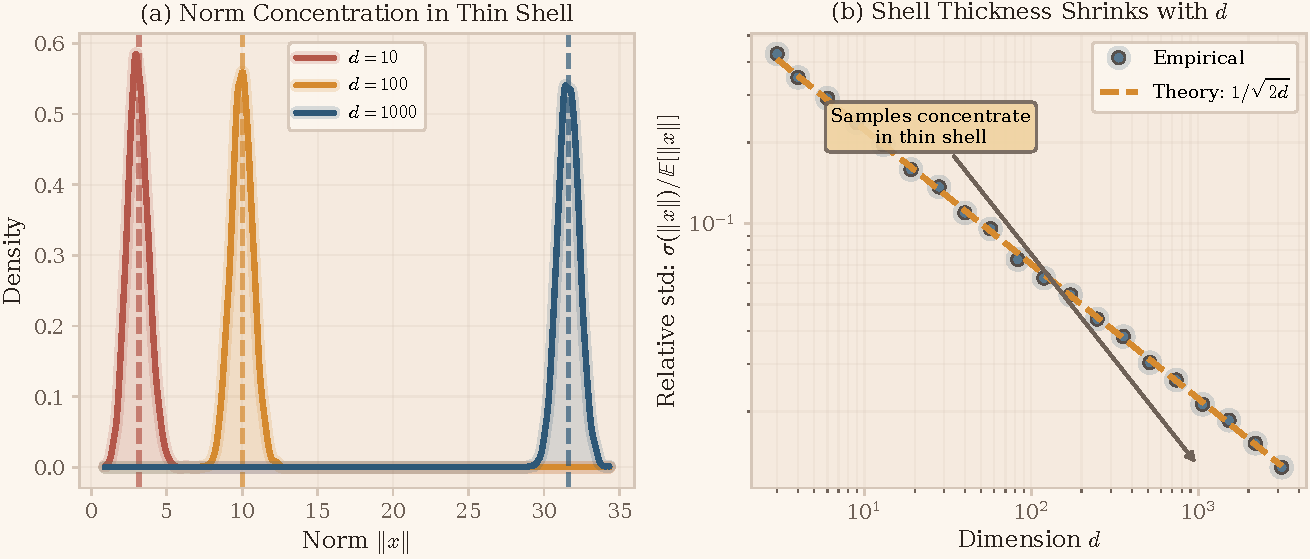
\includegraphics[width=\linewidth]{code/figures/ch04_highdim_representations/fig_4_4_gaussian_shell.pdf}
\caption{Gaussian thin shell: the norm concentrates near $\sqrt{d}$, and its relative spread scales as $1/\sqrt{2d}$, yielding an increasingly thin probabilistic shell.}
\label{fig:gaussian_shell}
\end{figure}

\vspace{1.5em}

Take another break. These concentration phenomena are the foundation of high-dimensional probability. Volume near surface, orthogonality of random vectors, uniformity of distances, and typicality. These are not edge cases. They are the typical behavior in high dimensions.

\vspace{2em}

%==========================
\section[Random Projections and the Johnson--Lindenstrauss Lemma]{Random Projections and the\texorpdfstring{\\}{ }Johnson--Lindenstrauss Lemma}

\subsection{Can You Compress Without Losing Information?}

Here is a practical question. You have data in a very high-dimensional space, say $d = 10{,}000$ dimensions. Can you project it down to a much lower-dimensional space, say $k = 100$ dimensions, without losing much information?

Intuitively, this seems impossible. You are throwing away 99\% of the dimensions. How could distances and relationships be preserved?

But here is the magic: if you have a finite set of points, you can compress them with minimal distortion using random projections. This is the content of the Johnson--Lindenstrauss lemma.

\vspace{1.5em}

\subsection{The Johnson--Lindenstrauss Lemma}
\label{sec:jl}

The Johnson--Lindenstrauss (JL) lemma says: for any set of $n$ points in high-dimensional space, there exists a projection to $k = O(\log n / \epsilon^2)$ dimensions such that all pairwise distances are preserved up to a factor of $(1 \pm \epsilon)$.

More precisely, there exists a linear map $f: \mathbb{R}^d \to \mathbb{R}^k$ such that for all pairs of points $x, y$:

\begin{equation}
(1-\epsilon)\|x - y\|^2 \leq \|f(x) - f(y)\|^2 \leq (1+\epsilon)\|x - y\|^2
\end{equation}

The remarkable part is that $k$ depends only on $n$ (the number of points) and $\epsilon$ (the desired accuracy), not on $d$ (the original dimension). Even if $d = 1{,}000{,}000$, you can often project down to $k = O(\log n)$ and preserve distances for a fixed set of $n$ points.

More refined statements include a failure probability $\delta$ and yield $k = O(\log(n/\delta)/\epsilon^2)$.

\begin{figure}[t]
\centering
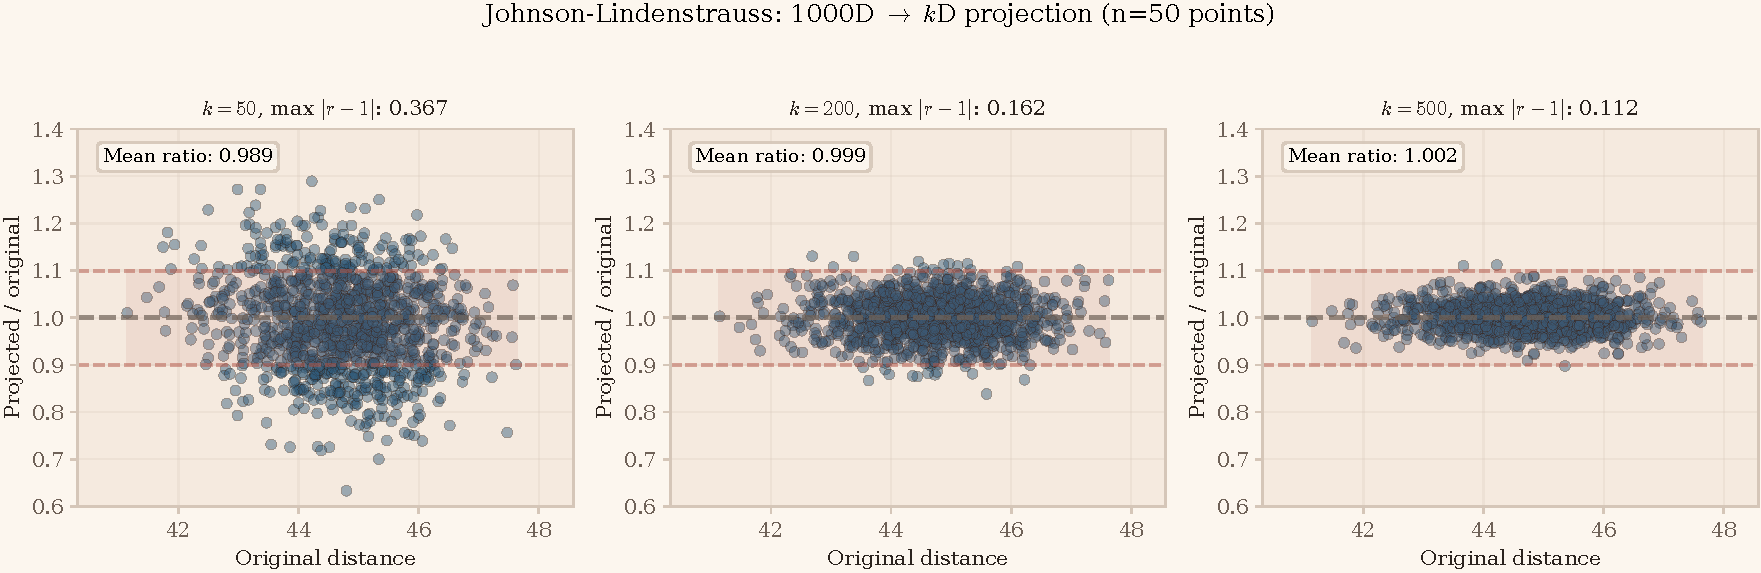
\includegraphics[width=\linewidth]{code/figures/ch04_highdim_representations/fig_4_5_johnson_lindenstrauss.pdf}
\caption{Johnson--Lindenstrauss in practice (toy $n=50$ points): distance ratios $\|Rx-Ry\|/\|x-y\|$ for $k\in\{50,200,500\}$ with $\pm10\%$ bands around 1; random projections preserve distances increasingly well as $k$ grows (once $k=O(\log n/\epsilon^2)$).}
\label{fig:jl}
\end{figure}

\vspace{1em}

Moreover, you can use a random projection. You do not need to carefully design $f$. Just sample a random matrix with appropriate properties (like Gaussian entries scaled by $1/\sqrt{k}$), and with high probability, it will preserve distances.

\subsection{Why Does This Work? A Proof Sketch}
\label{sec:jl-proof}

The intuition behind the Johnson--Lindenstrauss lemma comes from concentration of measure. Let me sketch why random projections preserve distances.

\vspace{1em}

Consider projecting a single vector $x$ with $\|x\| = 1$ onto a random $k$ dimensional subspace using a random matrix $R$ with i.i.d. Gaussian entries $\mathcal{N}(0, 1/k)$. The projected length squared is:

\begin{equation}
\|Rx\|^2 = \sum_{i=1}^k (R_i^\top x)^2
\end{equation}

Similarly, inner products are preserved in expectation and concentrate. For fixed $x,y$,
\begin{equation*}
\begin{aligned}
\mathbb{E}[(Rx)^\top (Ry)] &= x^\top y,\\
\operatorname{Var}((Rx)^\top (Ry)) &= O(1/k).
\end{aligned}
\end{equation*}
So for a \emph{fixed} pair, a tail bound gives a small distortion with high probability once $k=\Omega(\log(1/\delta)/\epsilon^2)$. The JL lemma then lifts this fixed-pair statement to a \emph{finite set of pairs} using a union bound.

Each term $R_i^\top x = \sum_{j=1}^d R_{ij} x_j$ is a weighted sum of Gaussian random variables. Since $\sum_j x_j^2 = 1$, we have:

\begin{equation}
\mathbb{E}[(R_i^\top x)^2] = \sum_{j=1}^d x_j^2 \mathbb{E}[R_{ij}^2] = \sum_{j=1}^d x_j^2 \cdot \frac{1}{k} = \frac{1}{k}
\end{equation}

So $\mathbb{E}[\|Rx\|^2] = k \cdot (1/k) = 1$. The projection preserves length in expectation!

\vspace{1em}

The variance of $\|Rx\|^2$ is $O(1/k)$ by standard concentration results. By Chebyshev's inequality or Chernoff bounds, for $k = \Omega(1/\epsilon^2)$, we have:

\begin{equation}
P(|\|Rx\|^2 - 1| > \epsilon) < \delta
\end{equation}

for some small failure probability $\delta$.

\vspace{1em}

Now we want to preserve all $\binom{n}{2}$ distances among a fixed set of points $\{x_1,\ldots,x_n\}$. It is enough to preserve the lengths of the $\binom{n}{2}$ difference vectors $x_i-x_j$, because for a linear map $f(x)=Rx$ we have $f(x_i)-f(x_j)=R(x_i-x_j)$. Using a union bound over all pairs:

\begin{equation}
k = O\left(\frac{\log n}{\epsilon^2}\right)
\end{equation}

suffices to ensure all distances are preserved with high probability. The $\log n$ factor comes from the union bound: we need the failure probability per pair to be $O(1/n^2)$, i.e. $\log(1/\delta) = O(\log n)$.

\vspace{1em}

This is why the dimension depends only logarithmically on the number of points, not on the original dimension. Random projections exploit the concentration of measure in high dimensions.

\vspace{1.5em}

\begin{examplebox}
\textbf{How many dimensions do you need?}

\vspace{0.5em}

Suppose you have $n = 1{,}000{,}000$ points (one million) and you want to preserve distances up to $\epsilon = 0.1$ (10\% distortion). How many dimensions $k$ do you need?

\vspace{0.5em}

The Johnson--Lindenstrauss scaling is:
\begin{equation*}
k = O\left(\frac{\log n}{\epsilon^2}\right).
\end{equation*}

For $n = 10^6$ and $\epsilon = 0.1$, $\log n \approx 13.8$ (natural log), so $k$ is on the order of a \emph{few thousand}. Constants and the desired failure probability $\delta$ can easily move this up by a factor of several, but the key point is the \emph{logarithmic} dependence on $n$, not the exact prefactor.

If the original space has $d = 100{,}000$ dimensions, even a target dimension in the low thousands is a huge compression while preserving distances approximately.

\vspace{0.5em}

If you relax the accuracy to $\epsilon = 0.2$ (20\% distortion):
\begin{equation*}
k = O\left(\frac{\log n}{0.04}\right)
\end{equation*}

Because the bound scales like $1/\epsilon^2$, doubling $\epsilon$ cuts $k$ by about a factor of four (up to constants). Now you might get away with a few hundred dimensions.

\vspace{0.5em}

\textbf{Key insight:} The number of dimensions needed depends logarithmically on the number of points. Going from a million to a billion points only increases $\log n$ from about 13.8 to about 20.7 (a $\sim$1.5$\times$ factor). This is why random projections are so effective for high-dimensional data.
\end{examplebox}

\vspace{1.5em}

\subsection{Practical Applications of Random Projections}

Random projections are widely used in practice for dimensionality reduction:

\begin{itemize}
\item \textbf{Fast nearest neighbor search:} Project high-dimensional embeddings to lower dimensions, then search in the lower-dimensional space. This is much faster, and distances are approximately preserved.

\item \textbf{Sketching and streaming:} In large-scale data processing, you cannot store all data in memory. Random projections let you compute approximate statistics (like distances or inner products) using sketches that are much smaller than the original data.

\item \textbf{Obfuscation and privacy (informal):} A secret random projection can make raw features harder to interpret while approximately preserving geometry. This is \emph{not} a differential privacy guarantee without a clear threat model and added noise.

\item \textbf{Compressed sensing:} If a signal is sparse in some basis, you can recover it from far fewer measurements than the original dimension using random projections. This is the foundation of compressed sensing.
\end{itemize}

\vspace{1em}

The key advantage is that random projections are oblivious: you do not need to know anything about the data distribution. Just apply a random matrix, and distances are preserved with high probability. This makes them extremely practical.

\vspace{2em}

%==========================
\vspace{0.5em}

\textbf{Limits and failure modes.} Random projections are not a panacea.
\begin{itemize}
\item If you have an enormous number of points $n$, the required target dimension $k = O(\log n / \epsilon^2)$ can still be too large to be practical.
\item If your downstream task relies on \emph{structured correlations} (e.g., sparse, axis-aligned features or specific subspace arrangements), an oblivious projection can destroy that structure.
\item Some tasks truly need the full ambient geometry (e.g., exact ranking by tiny margin differences); a low-dimensional sketch may be insufficient.
\end{itemize}

\section{Tokenization and Embedding Geometry}

\subsection{From Discrete Symbols to Continuous Vectors}

Modern language models work with embeddings. Each token (word, subword, character) is mapped to a vector in a high-dimensional space, typically with $d = 768$ or $d = 1024$ or even higher dimensions.

This embedding space is where the model does its computation. Attention compares vectors. Feedforward layers transform vectors. The entire model operates in this continuous vector space, even though the input and output are discrete tokens.

\vspace{1em}

The geometry of this embedding space matters enormously. If semantically similar tokens have similar embeddings, the model can generalize. If the geometry is pathological (all embeddings point in the same direction, or the space is anisotropic), the model will struggle.

\vspace{1.5em}

\subsection{Tokenization: Breaking Text into Pieces}

Tokenization maps raw text to discrete symbols before embedding. In practice, modern systems use \emph{subword} schemes (e.g., BPE/WordPiece/SentencePiece) because they balance vocabulary size, sequence length, and coverage of rare or misspelled words. All you need for this chapter is the idea that tokens become vectors; the algorithmic details of tokenization and training belong with the Transformer architecture. See Chapter~5 for a focused treatment and practical guidance.

\vspace{1.5em}
\subsection{Anisotropy: When Embeddings Are Not Evenly Distributed}

Here is a problem that shows up in many trained embedding spaces: anisotropy. The embeddings are not uniformly distributed on the sphere. They concentrate in a narrow cone, pointing mostly in the same direction.

To quantify anisotropy, compute the average embedding vector:

\begin{equation}
\mu = \frac{1}{V} \sum_{i=1}^V e_i
\end{equation}

where $e_i$ is the embedding for token $i$ and $V$ is the vocabulary size. If embeddings are isotropic (evenly distributed), $\mu$ should be close to zero. But in practice, $\|\mu\|$ is often large, meaning all embeddings have a significant component pointing in the direction of $\mu$.

Mean shift is one common source of anisotropy, but not the only one. Even after centering, variance can be concentrated in a few directions (dominant principal components), which also inflates similarities and makes neighborhoods less discriminative.

\vspace{1em}

Why is this bad? Because the cosine similarity between two embeddings is:

\begin{equation}
\text{similarity}(e_i, e_j) = \frac{e_i^\top e_j}{\|e_i\| \|e_j\|}
\end{equation}

If both embeddings have a large component pointing in the direction of $\mu$, their dot product is dominated by this common component. The cosine similarity is always high, even for unrelated tokens. This makes similarity search less discriminative.

\vspace{1.5em}

\begin{examplebox}
\textbf{Anisotropy in word embeddings}

\vspace{0.5em}

Suppose embeddings are unit vectors, but they all share a large component in a common \emph{bias direction} $b$ (a unit vector, often close to $\mu/\|\mu\|$). Two embeddings $e_i$ and $e_j$ might look like:

\begin{equation*}
e_i = 0.8\, b + 0.6\, u_i, \quad e_j = 0.8\, b + 0.6\, u_j
\end{equation*}

where $u_i$ and $u_j$ are unit vectors orthogonal to $b$ (so they represent token-specific content). In high dimensions, unrelated directions are typically nearly orthogonal, so $u_i^\top u_j \approx 0$ for unrelated tokens.

\vspace{0.5em}

By Pythagoras, $\|e_i\|^2 = 0.8^2 + 0.6^2 = 1$, so the embeddings are normalized. The dot product is:
\begin{equation*}
e_i^\top e_j = (0.8\, b + 0.6\, u_i)^\top (0.8\, b + 0.6\, u_j) \approx 0.64 + 0 = 0.64
\end{equation*}

The cosine similarity is 0.64 (since embeddings are already normalized). This is high similarity, even though $u_i$ and $u_j$ are orthogonal (representing unrelated semantic content).

\vspace{0.5em}

Many unrelated pairs of embeddings have similarity around 0.64 because of the shared component along $b$. The discriminative part (the $u_i$ and $u_j$ components) contributes much less to the similarity. This makes the embedding space less useful for retrieval: everything looks similar to everything else.

\vspace{0.5em}

\textbf{Solution:} Mean-centering subtracts $\mu$ and removes the shared component (centering/de-biasing). If anisotropy persists because variance is concentrated in a few directions, you can also remove a few top principal components or apply whitening (next section). After centering and whitening, you typically re-normalize before cosine similarity. Similarities become more discriminative because they reflect token-specific components, not shared global structure.
\end{examplebox}

\begin{figure}[t]
\centering
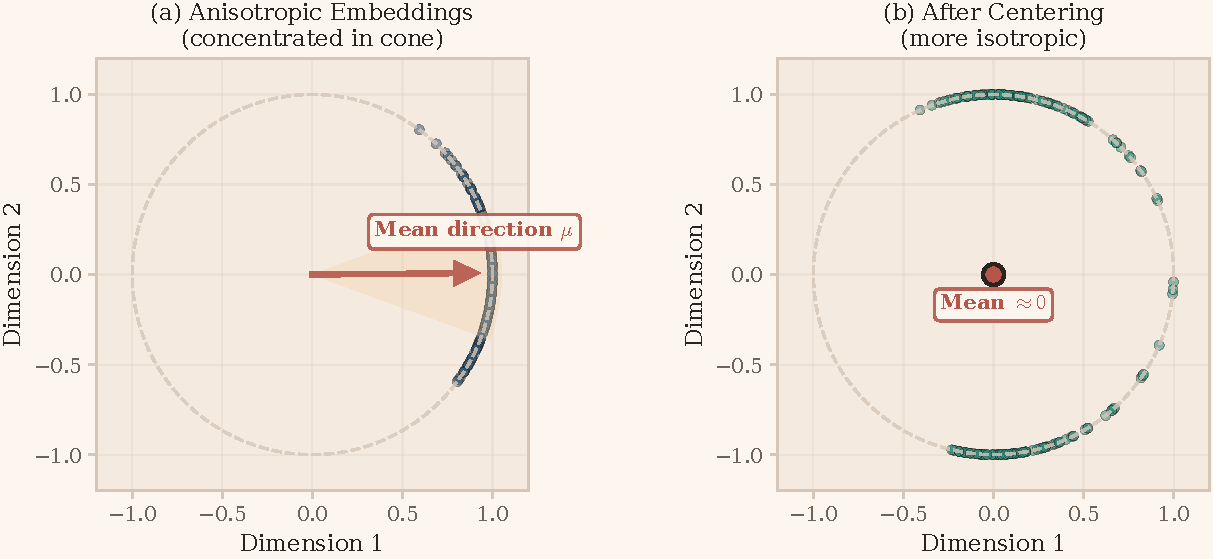
\includegraphics[width=\linewidth]{code/figures/ch04_highdim_representations/fig_4_6_anisotropy.pdf}
\caption{Embedding anisotropy: (a) unit-normalized tokens cluster in a narrow cone around a mean direction, inflating cosine similarities; (b) mean-centering spreads points and restores angular contrast.}
\label{fig:anisotropy}
\end{figure}

\vspace{1.5em}

\subsection{Whitening: Fixing the Geometry}

A more aggressive fix than centering is whitening. Whitening transforms the embeddings so that their covariance is the identity matrix. This makes the space isotropic: all directions have equal variance.

The whitening transformation is:

\begin{equation}
\tilde{e}_i = \Sigma^{-1/2}(e_i - \mu)
\end{equation}

where $\mu$ is the mean embedding and $\Sigma$ is the covariance matrix. The transformed embeddings $\tilde{e}_i$ have zero mean and identity covariance.

\vspace{0.5em}

\textbf{A brief PCA connection.} Principal components are the eigenvectors $U$ of $\Sigma$; the leading components (largest eigenvalues) are the directions of greatest variance and often carry salient semantics. Whitening rotates into this eigenbasis and rescales by $1/\sqrt{\lambda_i}$ so that all directions have unit variance. This is beneficial for \emph{retrieval} and similarity, but it can suppress frequency or magnitude cues that are useful in other tasks.

\vspace{0.5em}

\textbf{Practical note.} Full whitening requires estimating $\Sigma$ and applying a matrix square root, which can be expensive at scale. In practice, many retrieval systems use lighter-weight variants: mean-centering plus removing a few top principal components, or whitening computed on a representative sample of embeddings.

\textbf{Practical recipe (sampled whitening).} Compute $\mu$ on a large sample and center. Estimate $\Sigma$ on that sample and eigendecompose $\Sigma = U\,\mathrm{diag}(\lambda)\,U^\top$. Choose a small ridge $\varepsilon>0$ (to avoid exploding tiny-variance directions), then transform
\begin{equation*}
\tilde e = U\,\mathrm{diag}\!\left(\frac{1}{\sqrt{\lambda+\varepsilon}}\right)U^\top (e-\mu),
\end{equation*}
and (often) re-normalize $\tilde e$ if you are using cosine similarity.

\vspace{1em}

Whitening has two effects:

\begin{itemize}
\item It removes the common component (like centering)
\item It equalizes variance in all directions (removes dominant principal components)
\end{itemize}

\vspace{1em}

\begin{figure}[t]
\centering
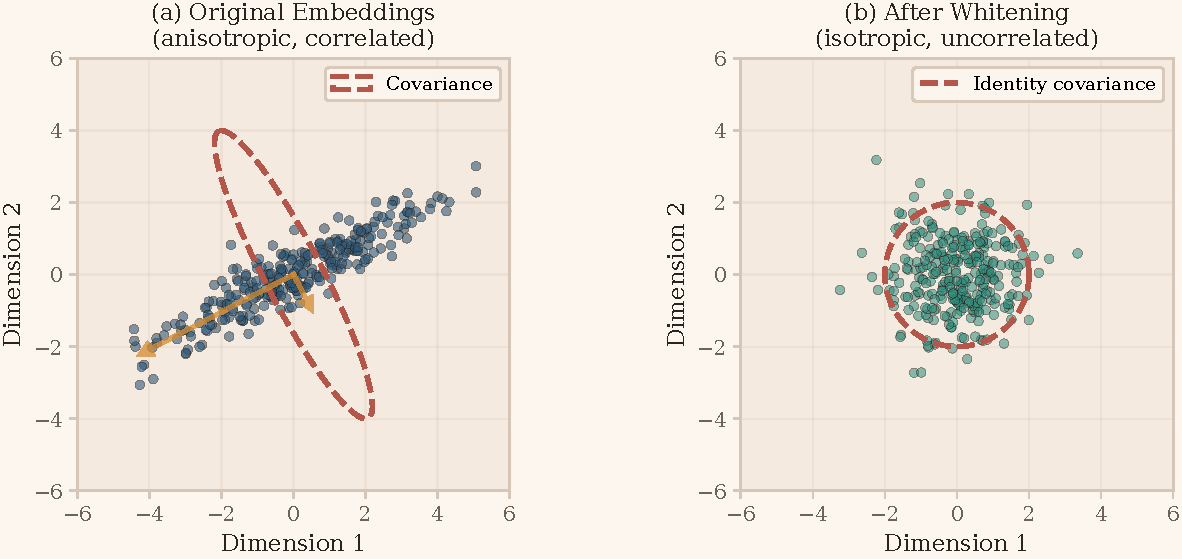
\includegraphics[width=\linewidth]{code/figures/ch04_highdim_representations/fig_4_7_whitening.pdf}
\caption{Whitening recenters and rescales embeddings via $\Sigma^{-1/2}(e-\mu)$ so that covariance becomes identity, making dimensions uncorrelated with equal variance and improving isotropy for similarity search.}
\label{fig:whitening}
\end{figure}

After whitening, cosine similarities are more evenly distributed. High similarity is less dominated by shared global components, and nearest neighbor search becomes more effective.

\vspace{1em}

However, whitening is not always beneficial. You should avoid whitening when:

\begin{itemize}
\item \textbf{Frequency information matters:} In some applications, common words should have larger magnitude to reflect their importance. Whitening destroys this signal.

\item \textbf{Principal components capture important semantics:} The dominant directions might encode meaningful structure like topic or sentiment. Whitening removes this structure by equalizing all directions.

\item \textbf{Embeddings are used for generation:} If you are sampling from the embedding space to generate text, the original distribution matters. Whitening changes the distribution and might make generation less coherent.
\end{itemize}

\vspace{1em}

\textbf{When to use whitening:} Primarily for retrieval tasks where only relative similarities matter. If you only care about ranking by similarity, whitening can substantially improve the discriminative power of your embeddings.

\vspace{1.5em}

\subsection{Subword Tokenization and Rare Token Problems}

Subword tokenization creates a challenge: rare tokens can have poor embeddings. Why? Because they appear infrequently in training data, so their embeddings are not well optimized. They end up in arbitrary positions, often far from semantically related tokens.

This affects performance on rare words, names, and domain-specific terms. The model sees these tokens rarely, so it cannot learn good representations.

\vspace{1em}

There are several approaches to mitigate this:

\begin{itemize}
\item \textbf{Character- or byte-level fallback:} If a token is rare, fall back to character- or byte-level encoding. This guarantees that every string can be represented, even if not optimally.

\item \textbf{Pretraining on diverse data:} Include data from many domains so that rare tokens in one domain are common in another. This helps the model learn better embeddings for a wider vocabulary.

\item \textbf{Subword pooling:} Represent rare words as combinations of their subword pieces. If "unbelievable" is broken into "un", "believ", "able", pool the embeddings of these pieces. This leverages compositionality.

\item \textbf{Fine-tuning embeddings:} If you have domain-specific data, fine-tune the embedding layer to improve representations for your specific vocabulary. This is especially useful for proper nouns and technical terms.
\end{itemize}

\vspace{2em}

Take a breath here. Tokenization and embeddings are the foundation of how models represent text. The geometry of the embedding space determines how well the model can capture semantic relationships. Anisotropy and rare token problems are real issues that you need to understand and address.

\vspace{2em}

%==========================
\section{Similarity Search and Information in Retrieval}

\subsection{Why Normalize to the Sphere?}

In many applications, embeddings are normalized to unit length. This projects them onto the unit sphere. Distances are then measured using cosine similarity:

\begin{equation}
\text{cosine}(u, v) = \frac{u^\top v}{\|u\| \|v\|} = u^\top v \text{ (if normalized)}
\end{equation}

Why do this? Because for many semantic tasks, the direction of the embedding matters more than its magnitude. "King" and "queen" should have similar directions even if their magnitudes differ slightly.

\vspace{1em}

Normalizing to the sphere also has computational benefits. Cosine similarity is just a dot product, which is fast. And you do not need to store or compute norms.

\vspace{1em}

\textbf{When to use L2 distance vs cosine similarity:}

\begin{itemize}
\item \textbf{Cosine similarity:} Use when direction matters more than magnitude. Typical for semantic similarity, document retrieval, and recommendation systems. Less sensitive to scale differences (a longer document should not automatically be more similar).

\item \textbf{L2 (Euclidean) distance:} Use when magnitude carries meaning. Typical for images (brightness matters), audio (volume matters), or when embeddings are calibrated so that magnitude encodes confidence or importance.
\end{itemize}

\vspace{1em}

In practice, for normalized embeddings, L2 distance and cosine similarity are monotonically related: $\|u - v\|^2 = 2(1 - u^\top v)$. So ranking by L2 distance gives the same order as ranking by cosine similarity.

\vspace{1.5em}

\subsection{Angular Distances and the Dot Product}

On the sphere, the natural distance is angular distance:

\begin{equation}
\theta = \arccos(u^\top v)
\end{equation}

This is the angle between the two vectors. If $\theta = 0$, they point in the same direction (identical). If $\theta = \pi/2$, they are orthogonal (unrelated). If $\theta = \pi$, they point in opposite directions (maximally dissimilar under cosine). In many learned embedding spaces, antonyms are \emph{not} reliably opposite; they often appear close because they share contexts.

For small angles, angular distance is approximately Euclidean distance:

\begin{equation}
\|u - v\|^2 = 2(1 - u^\top v) = 2(1 - \cos\theta) \approx \theta^2 \text{ for small } \theta
\end{equation}

So for nearby points on the sphere, angular distance and Euclidean distance are nearly the same. This is why many algorithms that assume Euclidean geometry still work reasonably well on the sphere.

\vspace{0.5em}

\textbf{Geometry intuition:} Angular distance is the geodesic on the sphere, while Euclidean distance is the straight chord in the ambient space (Figure~\ref{fig:spherical_geometry}).

\begin{figure}[ht]
\centering
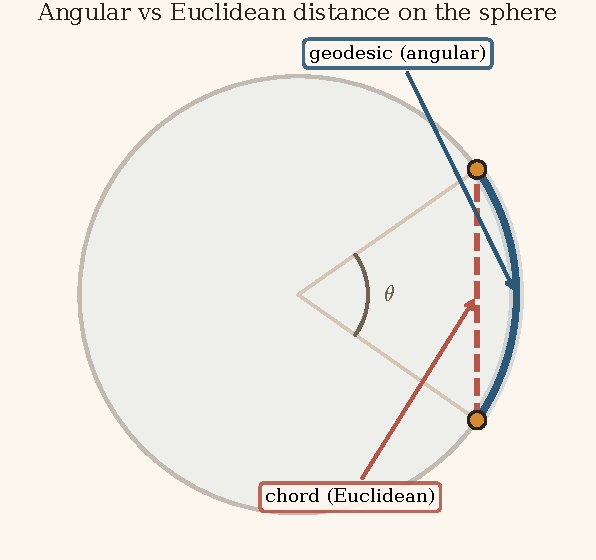
\includegraphics[width=0.88\linewidth]{code/figures/ch04_highdim_representations/fig_4_8_spherical_geometry.pdf}
\caption{Spherical geometry: the geodesic arc measures angular distance, while the straight chord is Euclidean distance in the ambient space. For small angles they agree; for large angles they diverge.}
\label{fig:spherical_geometry}
\end{figure}

\vspace{1.5em}

\begin{examplebox}
\textbf{Cosine similarity vs Euclidean distance}

\vspace{0.5em}

Suppose you have two normalized embeddings with cosine similarity $\cos\theta = 0.9$. What is the angular distance? What is the Euclidean distance?

\vspace{0.5em}

Angular distance:
\begin{equation*}
\theta = \arccos(0.9) \approx 0.451 \text{ radians} \approx 25.8 \text{ degrees}
\end{equation*}

Euclidean distance:
\begin{equation*}
\|u - v\|^2 = 2(1 - 0.9) = 0.2, \quad \|u - v\| \approx 0.447
\end{equation*}

Notice that the Euclidean distance 0.447 is close to the angular distance 0.451. This is the small angle approximation.

\vspace{0.5em}

Now suppose the cosine similarity is 0 (orthogonal). What are the distances?

\vspace{0.5em}

Angular distance:
\begin{equation*}
\theta = \arccos(0) = \pi/2 \approx 1.571 \text{ radians} \approx 90 \text{ degrees}
\end{equation*}

Euclidean distance:
\begin{equation*}
\|u - v\|^2 = 2(1 - 0) = 2, \quad \|u - v\| \approx 1.414
\end{equation*}

Now the Euclidean distance 1.414 is smaller than the angular distance 1.571. The small angle approximation breaks down.

\vspace{0.5em}

\textbf{Practical implication:} For highly similar embeddings (cosine close to 1), Euclidean distance and angular distance are nearly the same. For dissimilar embeddings, they diverge. If you need a proper spherical metric, angular distance is natural; for ranking, comparing dot products/cosines avoids computing $\arccos$.
\end{examplebox}

\vspace{1.5em}

\subsection{Spherical Codes: Packing Many Directions}

Once you normalize embeddings, you are effectively storing points on the unit sphere. This raises a natural question: \emph{how many vectors can you pack on the sphere while keeping them meaningfully separated?}

A \emph{spherical code} is a set of unit vectors $\{u_1,\ldots,u_M\}$ on $S^{d-1}$ with a minimum angular separation, for example $u_i^\top u_j \le \cos\theta$ for all $i\neq j$. Larger $\theta$ means better separation (less ``interference'' in dot products).

The key high-dimensional lesson is that you can pack \emph{exponentially many} nearly-orthogonal directions as $d$ grows. Intuitively, each stored vector excludes a ``spherical cap'' of nearby directions, and in high dimensions those caps occupy an exponentially tiny fraction of the surface area (another face of concentration of measure). This is one reason large vocabularies and large retrieval corpora can coexist with angular similarity: the space has enormous capacity in terms of well-separated directions.

This also connects to compression techniques like product quantization: quantization is effectively choosing a \emph{codebook} (a set of representative directions) and then encoding each vector by a short code that points to nearby codewords. Better codebooks correspond to better packings on the sphere (higher separation for a fixed size), which reduces collisions in similarity search.

\vspace{1.5em}

\subsection{Semantic Structure in Embedding Spaces}

High-quality embedding spaces have geometric structure that reflects semantic relationships. Some examples:

\begin{itemize}
\item \textbf{Clustering:} Semantically related words cluster together. All country names are in one region, all colors in another, all verbs in another.

\item \textbf{Linear substructures:} Relationships can be captured by vector arithmetic. The famous example is "king" minus "man" plus "woman" equals "queen." This suggests that gender is a linear direction in the space.

\item \textbf{Analogies:} If $a : b :: c : d$ (a is to b as c is to d), then $b - a \approx d - c$ in the embedding space. This captures relational similarity.
\end{itemize}

\vspace{1em}

These properties are not automatic. They emerge from training on large corpora with appropriate objectives. The distributional hypothesis ("words that occur in similar contexts have similar meanings") drives the geometry. Co-occurrence statistics shape the embedding space.

\vspace{1em}

However, not all structure is semantic. Some structure reflects frequency (common words cluster together), some reflects syntactic roles (nouns vs verbs), some reflects training artifacts. Interpreting embedding geometry requires care.

\vspace{1em}

\textbf{Connection to attention mechanisms:} In transformers, scaled dot-product attention compares query and key vectors via a dot product (with a $1/\sqrt{d_k}$ scaling to control magnitude). If vector norms are controlled (or vectors are normalized), this behaves similarly to cosine similarity; otherwise, norms also affect the score. Either way, attention performs a soft nearest neighbor lookup in representation space, retrieving information from positions with high similarity to the query.

\vspace{2em}

%==========================
\section{The k-NN Problem and Approximate Nearest Neighbors}

\subsection{Why Exact Search Is Expensive}

Given a query vector $q$ and a database of $n$ vectors in $\mathbb{R}^d$, find the $k$ nearest neighbors to $q$. This is the k-NN problem, and it is fundamental to many applications:

\begin{itemize}
\item \textbf{Retrieval augmented generation:} Find the most relevant documents for a query, then generate an answer using those documents.

\item \textbf{Recommendation systems:} Find items similar to what the user has liked in the past.

\item \textbf{Image search:} Find images similar to a query image based on embedding similarity.

\item \textbf{Anomaly detection:} Find the nearest normal examples to a test point. If the nearest neighbors are far away, the test point is anomalous.
\end{itemize}


Exact k-NN requires computing distances to all $n$ vectors, which is $O(nd)$ time (where $d$ is the dimension). For large $n$ (millions or billions) and large $d$ (hundreds or thousands), this is too slow.

So we use approximate nearest neighbors (ANN). The goal is to find vectors that are probably among the true k nearest neighbors, but with much less computation. You trade off recall (the fraction of true neighbors you find) for speed.

\vspace{1.5em}

\subsection{Why ANN Works Despite the Curse of Dimensionality}

Earlier we discussed how distances become uniform in high dimensions, which makes nearest neighbor search seem hopeless. Yet approximate nearest neighbor methods work well in practice. Why?

The key insight is that real data has structure:

\begin{itemize}
\item \textbf{Data lives on lower dimensional manifolds:} Natural images, text embeddings, and audio signals have intrinsic dimension much lower than the ambient dimension. The effective dimension might be 10 or 20, even if the embedding dimension is 1000.

\item \textbf{We accept approximate answers:} Exact nearest neighbors might not be necessary. Finding points that are close enough (say, in the top 10\% by distance) is often sufficient for applications.

\item \textbf{Indexing exploits local geometry:} Methods like HNSW build graphs that capture local neighborhood structure. They navigate from region to region, exploiting the fact that nearby points tend to cluster.

\item \textbf{Relative distances still carry information:} Even if absolute distances are concentrated, the ordering of a query's distances can still contain signal. ANN methods exploit this local ordering and often recover the top of the ranking without comparing everything.
\end{itemize}

\vspace{0.5em}

Figure~\ref{fig:manifold_structure} sketches a low-dimensional manifold embedded in a higher-dimensional space. Intrinsic coordinates straighten the surface, which is why local neighborhoods remain meaningful even when the ambient dimension is large.

\begin{figure}[ht]
\centering
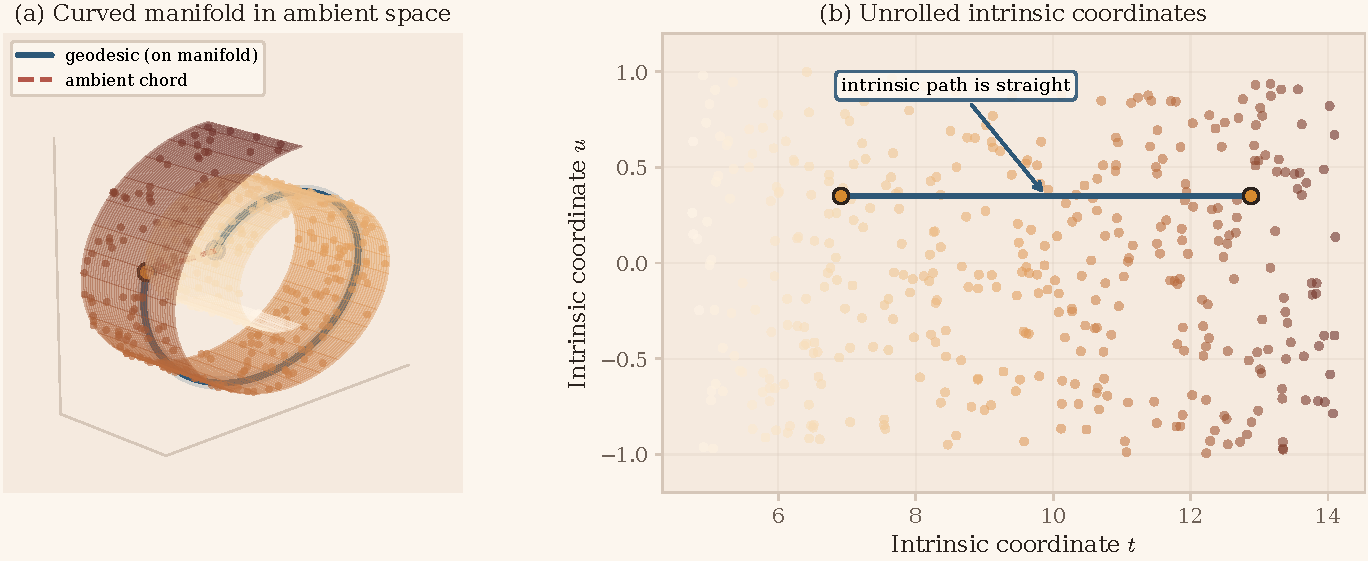
\includegraphics[width=0.95\linewidth]{code/figures/ch04_highdim_representations/fig_4_9_manifold_structure.pdf}
\caption{Low-dimensional manifold structure: (a) a curved surface embedded in a higher-dimensional ambient space; the intrinsic (geodesic) path follows the surface rather than the straight chord; (b) unrolled intrinsic coordinates straighten the manifold and make the path linear.}
\label{fig:manifold_structure}
\end{figure}

\vspace{1em}

This is why approximate nearest neighbor search is tractable despite the theoretical curse of dimensionality. The structure in real data makes the problem much easier than the worst case.

\vspace{1.5em}

\subsection{Indexing Structures for ANN}

There are many indexing structures for approximate nearest neighbor search:

\begin{itemize}
\item \textbf{Hierarchical navigable small world (HNSW):} Build a graph where each node is a vector and edges connect nearby vectors. Search by navigating the graph from a random starting point toward the query.

\item \textbf{Product quantization (PQ):} Compress vectors into short codes by clustering subspaces independently. Search by comparing codes instead of full vectors.

\item \textbf{Locality sensitive hashing (LSH):} Hash vectors so that nearby vectors hash to the same bucket with high probability. Search by checking buckets that the query hashes to.

\item \textbf{Inverted file index (IVF):} Partition the space into Voronoi cells using k-means clustering. Index vectors by which cell they belong to. Search by checking the cells nearest to the query.
\end{itemize}

\vspace{1em}

Each method has different tradeoffs between speed, memory, and recall, and which one is ``best'' depends on your constraints (latency, memory budget, update rate, and the similarity metric). Graph-based methods like HNSW often achieve excellent recall at low latency on many embedding workloads, but they can be memory-hungry because they store a neighborhood graph. Cluster-based methods like IVF reduce candidates by coarse quantization and are often combined with PQ (IVF+PQ) to scale to very large databases. PQ itself is extremely memory efficient and can make distance evaluation fast, but quantization introduces distortion; in practice you often rerank a small candidate set with the original vectors to recover recall. LSH has strong theoretical guarantees and can be very fast, but on dense learned embeddings its recall/latency tradeoff is often less competitive than graph- or cluster-based methods.

\vspace{1.5em}

\subsection{Product Quantization: Compressing Embeddings}

Product quantization deserves special attention because it achieves impressive compression while maintaining good search quality. The key idea is to split the $d$ dimensional vector into $m$ subspaces (typically choosing $m$ so that $d$ is divisible by $m$), then quantize each subspace independently.

\vspace{1em}

Here is how it works:

\begin{enumerate}
\item Split each vector $x \in \mathbb{R}^d$ into $m$ subvectors: $x = [x_1, x_2, \ldots, x_m]$ where each $x_i \in \mathbb{R}^{d/m}$.

\item For each subspace $i$, run k-means clustering with $k = 256$ clusters (so we can represent the cluster ID with 8 bits). This gives us $m$ codebooks, each with 256 centroids.

\item Represent each vector by its $m$ cluster IDs, one per subspace. This takes $m \times 8$ bits total.

\item To compute distance to a query, precompute distances from the query's subvectors to all centroids in each codebook ($m \times 256$ distances). Then for any database vector represented by cluster IDs, look up the distances in these tables and sum them. This is much faster than computing the full distance in $d$ dimensions.
\end{enumerate}

\vspace{1em}

\textbf{Practical note.} This description assumes an equal split into $d/m$-dimensional blocks. If $d$ is not divisible by $m$, you can pad, use uneven block sizes, or just choose a nearby $m$ (common choices are 8 or 16 dimensions per subvector). Also note that the codebooks are shared across the whole database, so their memory overhead is usually tiny compared to storing millions of vectors. Finally, PQ works best when the subspaces are close to independent; in practice, rotating the space before quantization (often called OPQ) can reduce cross-dimension correlation and improve accuracy.

\vspace{1em}

The compression ratio is $(d \times 32) / (m \times 8) = 4d/m$ \emph{assuming 32-bit (4-byte) floats for the original vectors and 8-bit (1-byte) codes per subvector}. For $d = 768$ and $m = 96$ (8 dimensions per subspace), the compression is $4 \times 768 / 96 = 32$ times. You store \textbf{96 bytes} of codes per vector instead of \textbf{3072 bytes}.

\vspace{1em}

The approximation error comes from quantization: each subvector is replaced by its nearest centroid, which introduces distortion. But because subspaces are quantized independently and the distortions average out, the overall distance approximation is often quite accurate.

\begin{figure}[t]
\centering
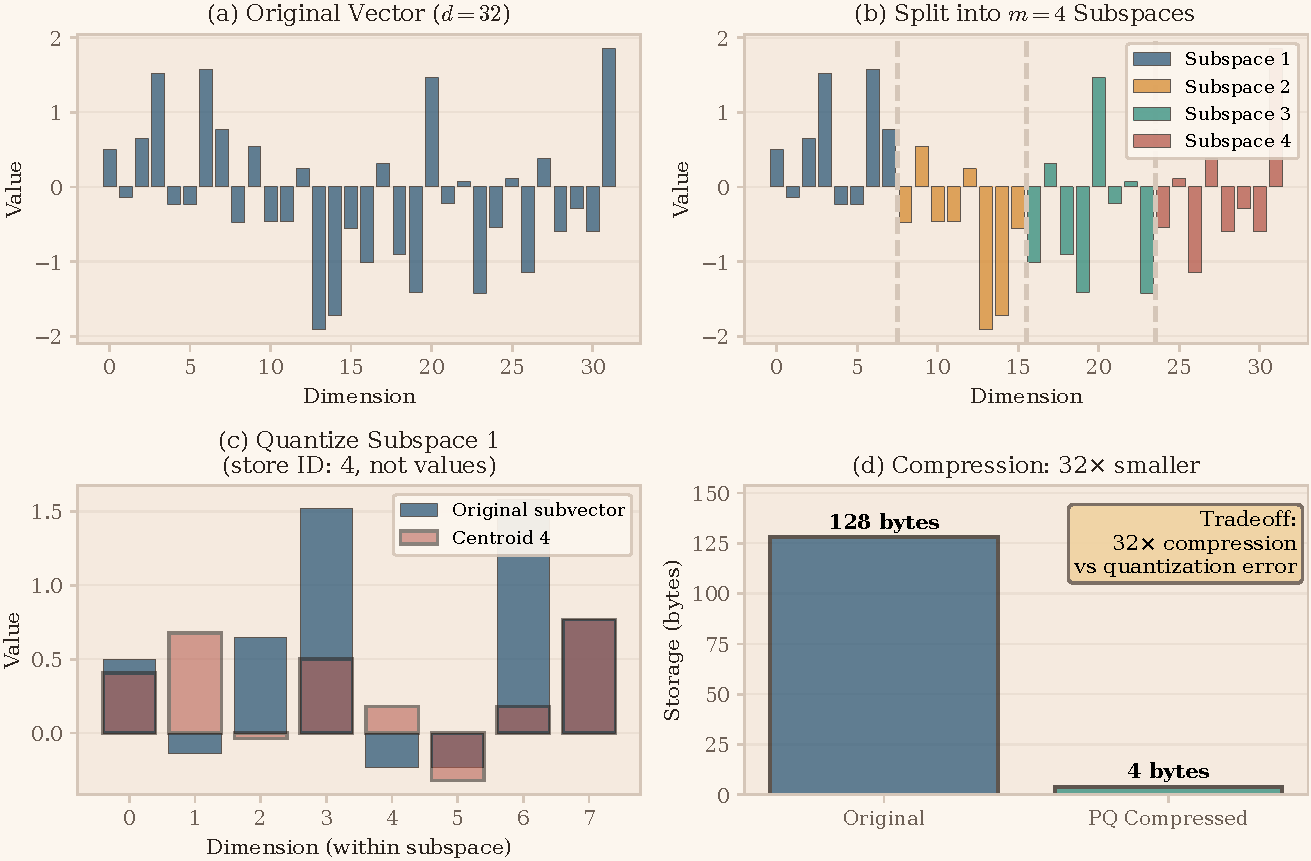
\includegraphics[width=\linewidth]{code/figures/ch04_highdim_representations/fig_4_10_product_quantization.pdf}
\caption{Product quantization (PQ): (a) a vector; (b) split into $m$ subspaces; (c) quantize each subspace with a small codebook and store centroid IDs; (d) toy compression example with $d=32$, $m=4$ (128 bytes $\rightarrow$ 4 bytes, 32$\times$) showing the compression--error tradeoff.}
\label{fig:product_quantization}
\end{figure}

\vspace{1.5em}

\subsection{Information-Theoretic View of Retrieval}

Retrieval can be viewed through an information-theoretic lens. The query $q$ provides information about which vectors in the database are relevant. The goal is to use this information efficiently to locate the relevant vectors.

Each comparison (computing a distance, checking a bucket, following a graph edge) gives you some information, though it is not a clean independent ``bit.'' Still, there is a useful counting intuition: to name one item out of $n$ you need at least $\log_2 n$ bits of information, so any retrieval method needs at least that much signal from the query and the index.

\vspace{1em}

A perfect binary search would find the nearest neighbor with $\log_2 n$ comparisons. But binary search requires a total ordering, which does not exist for vectors in high dimensions. So we need more comparisons.

Approximate nearest neighbor algorithms use indexing structures to reduce the number of comparisons. They are a form of lossy compression: you do not get the exact nearest neighbor, but you get a good approximation with far less work.

\vspace{1em}

Recall from Chapter 1 that rate distortion theory formalizes the tradeoff between compression and accuracy. Retrieval is an instance of this tradeoff: you compress the search space (by using an index, by quantizing vectors, by approximating distances), and you accept some distortion (loss of recall) in exchange for faster search (lower ``rate,'' often proxied by comparisons/work).

\vspace{1.5em}

\begin{examplebox}
\textbf{Information cost of k-NN search}

\vspace{0.5em}

Suppose you have a database of $n = 1{,}000{,}000$ vectors and you want to find the $k = 10$ nearest neighbors to a query.

\vspace{0.5em}

\textbf{Brute force search:}

Compute distance to all $n$ vectors. If each distance computation takes 1 unit of work, total cost is $n = 1{,}000{,}000$ units.

\vspace{0.5em}

\textbf{HNSW index:}

Build a multi-layer graph (roughly logarithmic depth). A typical query visits on the order of a few hundred to a few thousand nodes, depending on parameters and the target recall. As a concrete number, call it 1000 distance computations.

This is a speedup of $1{,}000{,}000 / 1000 = 1000$ times. You pay a cost in memory (storing the graph) and a small loss in recall (you might miss some true neighbors).

\vspace{0.5em}

\textbf{Product quantization:}

Compress each vector from $d = 768$ dimensions (using 4 bytes per dimension, so 3072 bytes) to a code of length 96 bytes (compression ratio of 32).

Distance computations on codes are much faster (looking up precomputed tables instead of computing full distances in $d$ dimensions). The speedup can easily be \emph{tens of times} for distance evaluation, plus the compression saves memory.

However, quantization introduces errors. The compressed distance is an approximation to the true distance, so recall drops (you might retrieve slightly wrong neighbors).

\vspace{0.5em}

\textbf{Information theoretic view (informal):} The lower bound is still $\log_2 n = 20$ bits to name one neighbor out of $n$. To name an \emph{unordered} set of $k$ neighbors, a more precise counting baseline is $\log_2 \binom{n}{k}$ bits (which is roughly $k\log_2 n$ when $k \ll n$), so for $k=10$ it is on the order of a couple hundred bits. Real ANN algorithms do not literally achieve this bound because comparisons are noisy/correlated and geometry does not induce a total order, but the point is that good indexes push query cost much closer to logarithmic than linear in $n$.
\end{examplebox}

\vspace{1.5em}

\subsection{Recall and Precision as Information Measures}

To evaluate an ANN system, fix a query $q$ and define:
\begin{itemize}
\item the \textbf{true top-$k$ neighbor set} $N_k(q)$ (the $k$ closest database vectors under your chosen metric),
\item the \textbf{returned set} $\hat N_k(q)$ produced by your index.
\end{itemize}

\vspace{0.5em}

Then the standard top-$k$ metrics are:
\begin{itemize}
\item \textbf{Recall@k:} $\mathrm{recall@k}(q) = \frac{|N_k(q) \cap \hat N_k(q)|}{k}$.
\item \textbf{Precision@k:} $\mathrm{precision@k}(q) = \frac{|N_k(q) \cap \hat N_k(q)|}{|\hat N_k(q)|}$.
\end{itemize}

\vspace{0.75em}

If your system always returns exactly $k$ items, then $|\hat N_k(q)| = k$ and \textbf{precision@k equals recall@k}. This is why ANN benchmarks often report just \emph{recall@k}: it directly answers ``how many of the true top-$k$ did we recover?'' (and you typically average it over many queries).

\vspace{0.75em}

In document retrieval, ``relevant'' is usually defined by labels or human judgment rather than ``true nearest neighbors,'' and you may return a variable number of items (or sweep a similarity threshold). In that setting, precision and recall differ, and you can trade one for the other, producing a precision--recall curve.

\vspace{1em}

In the exact case, recall@k is 100\%. In approximate search, you trade off recall for speed: higher recall typically costs more computation. Informally, recall is a proxy for how much information your retrieval system preserves about the true neighbor set. This is the same structure as rate distortion theory from Chapter 1: you compress the database into an index (lower ``rate,'' fewer comparisons/work) and you accept some distortion (missed neighbors) in exchange for faster search.

\vspace{2em}

%==========================

\begin{geometrylens}
\textbf{Voronoi Cells and Space Partitioning}

\vspace{0.5em}

Many indexing structures for nearest neighbor search are based on partitioning the space into cells. Each cell contains a cluster of nearby vectors. To search, you identify which cells the query is close to, then search within those cells.

\vspace{0.5em}

The most common partitioning is Voronoi cells. Given a set of centroids $c_1, \ldots, c_m$, the Voronoi cell for $c_i$ is the set of all points that are closer to $c_i$ than to any other centroid:

\begin{equation*}
V_i = \{x : \|x - c_i\| \leq \|x - c_j\| \text{ for all } j\}
\end{equation*}

Voronoi cells partition the space into convex polytopes. Each cell has a single centroid, and all points in the cell are closest to that centroid.

\vspace{0.5em}

IVF (inverted file index) uses Voronoi cells. You cluster the database vectors using k-means to get $m$ centroids. Each vector is assigned to the nearest centroid. At query time, you find the nearest centroids to the query and search the vectors in those cells.

\vspace{0.5em}

The geometry of Voronoi cells determines recall. If cells are small (many centroids), the query might span multiple cells, and you need to search multiple cells to get high recall. If cells are large (few centroids), each cell contains many vectors, and search within a cell is slow.

\vspace{0.5em}

There is a tradeoff between how many cells you create and how many cells you probe at query time. With few centroids, each cell is large, so searching a cell means evaluating many candidates (slow, but often high recall). With many centroids, each cell is smaller, but you may need to probe multiple nearby cells to maintain recall; probing too few cells can miss true neighbors.
\end{geometrylens}

\vspace{2em}

%==========================

\begin{pausebox}
Let me check your understanding. Can you explain why high-dimensional balls are hollow (most volume near the surface)? Do you understand why random vectors in high dimensions are nearly orthogonal? Can you state the Johnson--Lindenstrauss lemma and explain intuitively why it works (projection preserves length in expectation, concentration ensures small variance)?

\vspace{0.5em}

Can you explain what anisotropy is in embedding spaces and why it is a problem? Do you understand the difference between centering and whitening, and when you would use each? Can you explain why cosine similarity is used for normalized embeddings, and how it relates to angular distance?

\vspace{0.5em}

Can you articulate the tradeoff between recall and speed in approximate nearest neighbor search? Do you understand why ANN works despite the curse of dimensionality (data structure, approximate answers, local geometry)? Can you explain how product quantization achieves compression and why it introduces distortion?

\vspace{0.5em}

If any of these feel unclear, revisit the relevant section. High-dimensional geometry is counterintuitive, and it is worth spending time to build solid intuition. These concepts underlie all modern embedding-based systems, from language models to image search to recommendation engines.
\end{pausebox}

\vspace{1em}

This chapter explored the strange and wonderful world of high-dimensional representations. We learned about concentration of measure: how volume concentrates near the surface of balls, how random vectors are nearly orthogonal, and how distances concentrate. We saw the Johnson--Lindenstrauss lemma, which says you can compress high-dimensional data with minimal distortion using random projections, and we sketched why it works through concentration of measure. We dove into tokenization and embedding geometry, understanding anisotropy and how centering/whitening can improve retrieval geometry (with tradeoffs). We explored cosine similarity and angular distance on the sphere, and we introduced spherical codes as a way to think about packing many well-separated directions. Finally, we connected information theory to similarity search, viewing retrieval as lossy compression with a tradeoff between recall and speed.

High-dimensional geometry is not intuitive, but it is essential for working with modern AI systems. Embeddings are the lingua franca of machine learning: everything becomes vectors, and all operations are geometric. Understanding the properties of these spaces, their pathologies and their structure, is what separates practitioners who use embeddings blindly from those who use them effectively.

In the next chapter, we will turn to models themselves. We will see transformers as conditional compressors, understanding autoregression through the lens of incremental codelength minimization. The information-theoretic and geometric foundations we have built will illuminate how transformers work and why they succeed, and we will see how attention mechanisms perform soft nearest neighbor lookups in embedding space using dot-product similarity.
